% Chapter 3

\chapter{Analyzer Overview} % Main chapter title

\label{Chapter3}

\section{Theoretical Construction}
The development of our tool followed a structured, multi-step approach. As outlined in \capref{Chapter1}, to assess comment quality, it was necessary to categorize comments based on specific criteria, as illustrated in the figure below.

\begin{figure}[ht]
	\centering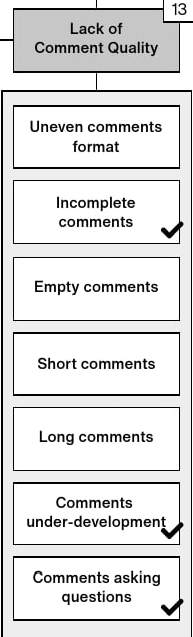
\includegraphics[height=350pt]{figs/goal-schema.PNG}
	\captionsetup{justification=centering}
	\caption{Comment categories the tool must be able to identify.}
	\label{fig:goal-schema}
\end{figure}

\noindent We began with simpler detections, such as identifying empty comments and comments that posed questions. Established rules were applied to determine if a comment was empty or contained either direct or implied questions.

\noindent Next, we tackled short and long comments. To achieve this, we utilized the \href{https://www.nltk.org/}{Natural Language Toolkit (NLTK)}, a comprehensive suite for natural language processing. By tokenizing each comment, we measured its length to classify it as either too short or overly long.

\noindent For comments under development, we employed pattern recognition techniques. We incorporated technical keywords and common phrases used during development to detect these comments.

\noindent The detection of incomplete comments and uneven comments format was refined through an iterative trial-and-error process, manually verifying results at each step. For incomplete comments, we initially performed a syntactic analysis to ensure the comments adhered to basic rules of English sentence structure. Subsequently, we built a classification system to categorize comments as single-line, multi-line, or documentation. For documentation comments, we verified consistency between the number of parameters in the comment and the corresponding source code, along with matching return types. Additionally, we introduced checks for single-line and multi-line comments to identify nonsensical or "gibberish" content, hence marking those that lacked clarity or coherence as incomplete.

\noindent Finally, for detecting uneven formatting, we flagged comments with irregular indentation, spacing, or annotation tag misuse, tailored to the programming language in use. This ensured that comments maintained proper structure, readability, and compliance with language-specific conventions.
